\documentclass[fleqn]{article}
\usepackage[utf8]{inputenc}
\usepackage[margin=2.5cm]{geometry}

% tikz
\usepackage{tikz}
\usetikzlibrary{positioning}

% maths / theorems
\usepackage{amsmath}
\usepackage{amssymb}
\usepackage{bm}

\begin{document}
\begin{figure}
\centering
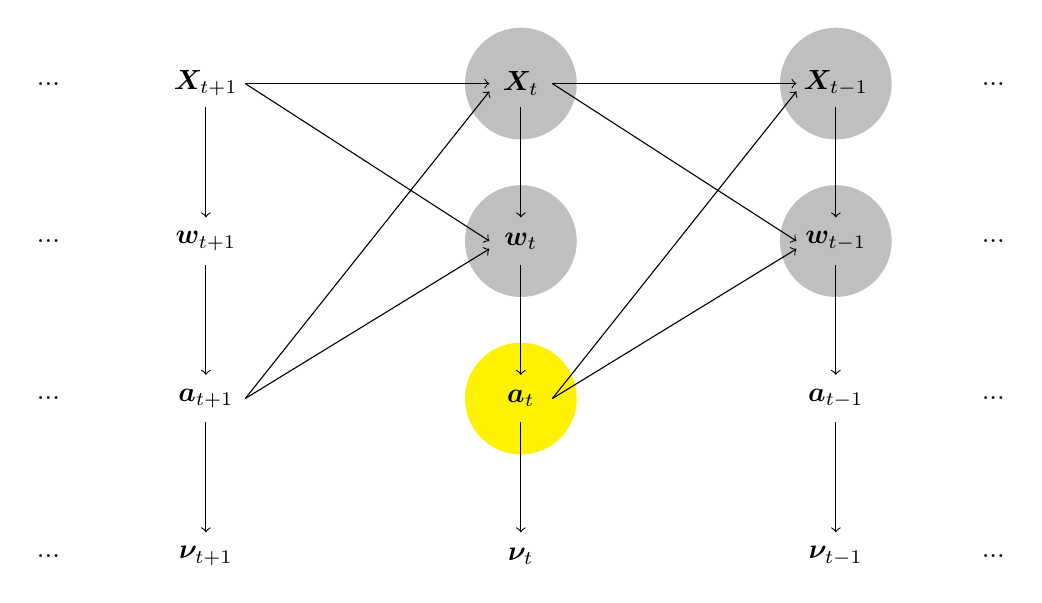
\begin{tikzpicture}
%%% Draw on filtration (F_t) as nested areas...
% highlighting circles
\filldraw[lightgray] (4,0) circle (20pt);
\filldraw[lightgray] (8,0) circle (20pt);
\filldraw[lightgray] (4,-2) circle (20pt);
\filldraw[lightgray] (8,-2) circle (20pt);
\filldraw[yellow] (4,-4) circle (20pt);
% left dots
\node at (-2,0) {...};
\node at (-2,-2) {...};
\node at (-2,-4) {...};
\node at (-2,-6) {...};
% labels (t+1)
\node at (0,0) {$\bm{X}_{t+1}$};
\node at (0,-2) {$\bm{w}_{t+1}$};
\node at (0,-4) {$\bm{a}_{t+1}$};
\node at (0,-6) {$\bm{\nu}_{t+1}$};
% labels t
\node at (4,0) {$\bm{X}_{t}$};
\node at (4,-2) {$\bm{w}_{t}$};
\node at (4,-4) {$\bm{a}_{t}$};
\node at (4,-6) {$\bm{\nu}_{t}$};
% labels (t-1)
\node at (8,0) {$\bm{X}_{t-1}$};
\node at (8,-2) {$\bm{w}_{t-1}$};
\node at (8,-4) {$\bm{a}_{t-1}$};
\node at (8,-6) {$\bm{\nu}_{t-1}$};
% right dots
\node at (10,0) {...};
\node at (10,-2) {...};
\node at (10,-4) {...};
\node at (10,-6) {...};
% arrows (t+1) -> t
\draw[->] (0.5,0)--(3.6,0);
\draw[->] (0.5,0)--(3.6,-2);
\draw[->] (0.5,-4)--(3.6,-2.1);
\draw[->] (0.5,-4)--(3.6,-0.1);
% arrows t -> (t-1)
\draw[->] (4.4,0)--(7.5,0);
\draw[->] (4.4,0)--(7.5,-2);
\draw[->] (4.4,-4)--(7.5,-2.1);
\draw[->] (4.4,-4)--(7.5,-0.1);
% vertical arrows (t+1)
\draw[->] (0,-0.3)--(0,-1.7);
\draw[->] (0,-2.3)--(0,-3.7);
\draw[->] (0,-4.3)--(0,-5.7);
% vertical arrows t
\draw[->] (4,-0.3)--(4,-1.7);
\draw[->] (4,-2.3)--(4,-3.7);
\draw[->] (4,-4.3)--(4,-5.7);
% vertical arrows (t-1)
\draw[->] (8,-0.3)--(8,-1.7);
\draw[->] (8,-2.3)--(8,-3.7);
\draw[->] (8,-4.3)--(8,-5.7);
\end{tikzpicture}
\caption{Part of the conditional independence graph for Algorithm [1]. The forwards direction of time is from left to right. Nodes highlighted in grey form the separatrix $\mathcal{H}_t$ which separates $\bm{a}_t$ (highlighted in yellow) from $\mathcal{F}_{t-1}$.}
\end{figure}
\end{document}